\chapter{Appendice}

\section{Componenti hardware utilizzati}
Il sistema \textit{Smart Garage Door} è stato realizzato utilizzando esclusivamente componenti open source e a basso costo.  
La Tabella~\ref{tab:hardware} elenca i principali elementi hardware con le relative funzioni e stime di costo.

\begin{table}[h!]
\centering
\caption{Elenco componenti hardware e costi}
\label{tab:hardware}
\begin{tabularx}{\textwidth}{@{}lXc@{}}
\toprule
\textbf{Componente} & \textbf{Funzione principale} & \textbf{Costo (€)} \\
\midrule
Arduino Nano & Controllo locale, gestione PIR e relè & 12.00 \\
NodeMCU ESP8266 & Gateway Wi-Fi, pubblicazione MQTT, bridge con server & 10.50 \\
Modulo GPS & Rilevazione posizione utente per automazione di prossimità & 14.00 \\
Sensore PIR & Rilevamento movimento per apertura automatica in uscita & 6.00 \\
Modulo relè 5V & Attuazione comando elettrico del motore porta & 5.00 \\
Breadboard e cablaggi & Collegamenti di prototipazione e alimentazione & 8.00 \\
Alimentatore 5V / 2A & Alimentazione microcontrollori e sensori & 7.50 \\
Materiali vari (case, connettori, staffe) & Supporti meccanici e alloggiamento & 7.00 \\
\midrule
\textbf{Totale stimato} & & \textbf{70–90 €} \\
\bottomrule
\end{tabularx}
\end{table}

Il costo complessivo rimane ampiamente entro il limite imposto dal requisito NFR10 (\textit{costo inferiore 150 €}), lasciando margine per futuri upgrade o sensori aggiuntivi.

\section{Software e librerie impiegate}
Tutti i software e le librerie utilizzate sono open source e compatibili con piattaforme multipiattaforma.  
La Tabella~\ref{tab:software} riassume le principali dipendenze software.

\begin{table}[h!]
\centering
\caption{Librerie e strumenti software utilizzati}
\label{tab:software}
\begin{tabularx}{\textwidth}{@{}lX@{}}
\toprule
\textbf{Libreria / Strumento} & \textbf{Funzione} \\
\midrule
\texttt{Arduino IDE 2.3} & Ambiente di sviluppo per microcontrollori Arduino e NodeMCU \\
\texttt{PubSubClient} & Implementazione client MQTT per ESP8266 \\
\texttt{SoftwareSerial} & Comunicazione seriale tra Arduino e NodeMCU \\
\texttt{TinyGPSPlus} & Calcolo distanza e coordinate da modulo GPS \\
\texttt{Flask 3.0} & Web framework per server locale in Python \\
\texttt{requests} & Gestione delle comunicazioni HTTP client-server \\
\texttt{Telebot / python-telegram-bot} & Interfaccia bot Telegram per comandi e notifiche \\
\texttt{ThingSpeak API} & Piattaforma MQTT per raccolta e visualizzazione dati \\
\texttt{Matplotlib / Pandas} & Analisi e rappresentazione grafica dei log sperimentali \\
\bottomrule
\end{tabularx}
\end{table}

Tutte le librerie utilizzate rispettano licenze open source (MIT, BSD o GPL), garantendo riusabilità e pubblicazione accademica.

\section{Schema elettrico semplificato}
Il collegamento tra i moduli principali è riportato nello schema seguente, dove vengono evidenziate le connessioni di alimentazione e segnale.


\begin{figure}[h!]
    \centering
    \includegraphics[width=0.9\textwidth]{images/elettrical_scheme.pdf}
    \caption{Schema elettrico semplificato del sistema Smart Garage Door}
    \label{fig:schematic}
\end{figure}


Lo schema mostra le interfacce principali:
\begin{itemize}
    \item connessione seriale TX/RX tra Arduino e NodeMCU;
    \item alimentazione comune a 5\,V con ground condiviso;
    \item uscita digitale verso il relè;
    \item ingresso PIR con pin di interrupt.
\end{itemize}

\section{Struttura del codice sorgente}
Il codice del progetto è stato organizzato secondo la logica modulare mostrata in Figura~\ref{fig:code_structure}.  
Ogni componente è indipendente ma interconnesso tramite interfacce chiare e documentate.




\begin{figure}[H]
\centering
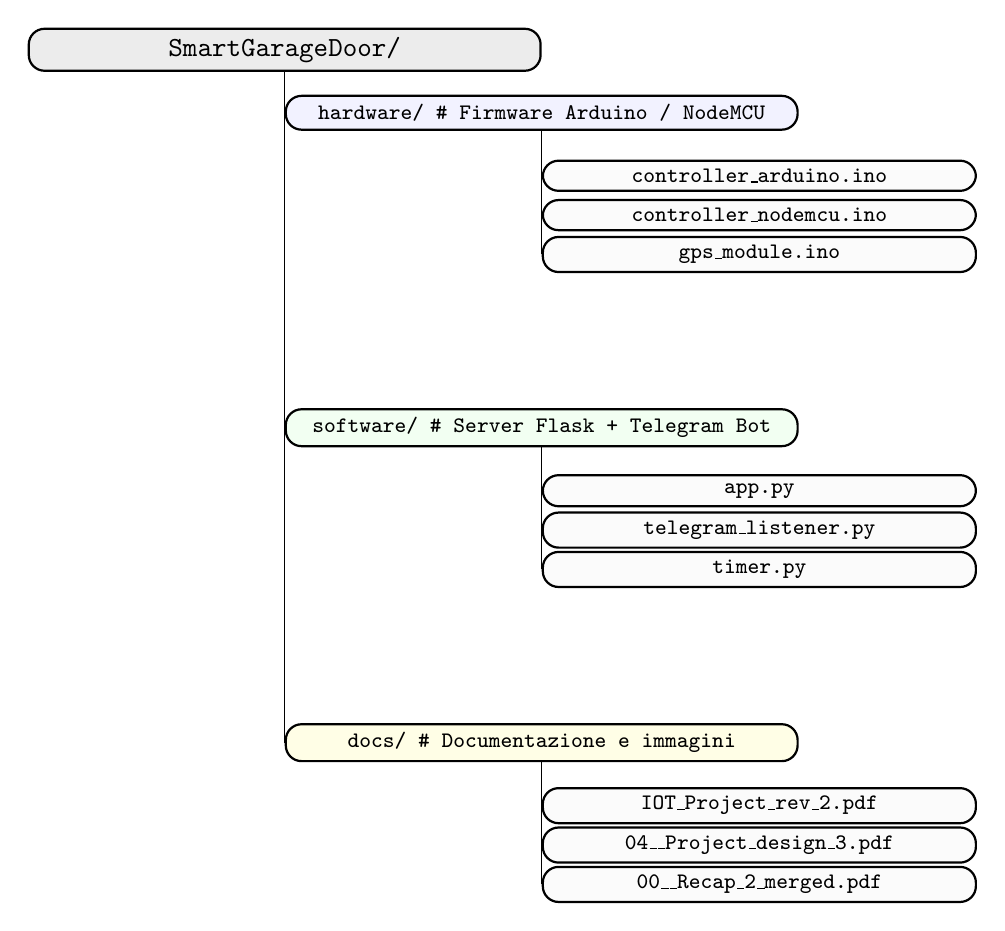
\begin{tikzpicture}[
  font=\footnotesize\ttfamily,
  level distance=8mm,
  sibling distance=0mm,
  grow=down,
  edge from parent path={(\tikzparentnode.south) -- ++(0,-2pt) -| (\tikzchildnode.west)},
  every node/.style={anchor=west, align=left},
  box/.style={draw, thick, rounded corners=2mm,
              minimum width=55mm, inner sep=3pt, fill=gray!3}
]

% Nodo principale
\node[box, fill=gray!15, font=\bfseries\ttfamily, minimum width=65mm]
  {SmartGarageDoor/}
  % ====================== HARDWARE ======================
  child { node[box, fill=blue!5!white, minimum width=65mm, yshift=0mm]
            {hardware/ \hfill \# Firmware Arduino / NodeMCU}
    child { node[box,yshift=0mm]   {controller\_arduino.ino} }
    child { node[box,yshift=-5mm]  {controller\_nodemcu.ino} }
    child { node[box,yshift=-10mm] {gps\_module.ino} }
  }
  % ====================== SOFTWARE ======================
  child { node[box, fill=green!5!white, minimum width=65mm, yshift=-40mm]
            {software/ \hfill \# Server Flask + Telegram Bot}
    child { node[box,yshift=0mm]   {app.py} }
    child { node[box,yshift=-5mm]  {telegram\_listener.py} }
    child { node[box,yshift=-10mm] {timer.py} }
  }
  % ====================== DOCS ======================
  child { node[box, fill=yellow!10!white, minimum width=65mm, yshift=-80mm]
            {docs/ \hfill \# Documentazione e immagini}
    child { node[box,yshift=0mm]   {IOT\_Project\_rev\_2.pdf} }
    child { node[box,yshift=-5mm]  {04\_\_Project\_design\_3.pdf} }
    child { node[box,yshift=-10mm] {00\_\_Recap\_2\_merged.pdf} }
  };

\end{tikzpicture}

\caption{Struttura delle directory e dei moduli principali del progetto \textit{Smart Garage Door}.  
Le tre sottocartelle principali — \texttt{hardware/}, \texttt{software/} e \texttt{docs/} — sono disposte verticalmente in modo proporzionato,  
ciascuna con i propri file allineati sullo stesso asse X per una rappresentazione chiara e leggibile.}
\label{fig:code_structure}
\end{figure}




\begin{itemize}
    \item \texttt{controller\_arduino.txt} – gestione sensori e relè, timer di chiusura automatica;
    \item \texttt{controller\_nodemcu.txt} – connessione MQTT e bridge seriale con Arduino;
    \item \texttt{Transmitter with Thingspeak.txt} – gestione GPS e pubblicazione distanza;
    \item \texttt{app.py} – server Flask, login, API e gestione comandi;
    \item \texttt{telegram\_listener.py} – interfaccia utente Telegram e notifiche;
    \item \texttt{timer.py} – controllo temporale e reset automatico stato.
\end{itemize}

\section{Esempi di log e output}
Durante i test sperimentali, i messaggi di stato generati dai vari moduli hanno confermato la coerenza tra eventi e comandi.  
Un estratto di log tipico è mostrato di seguito:

\begin{verbatim}
[NodeMCU] Connected to broker mqtt://192.168.1.4
[Arduino] PIR detected motion -> Door opening
[Flask] User lello issued command /on
[Telegram] Notification sent: Door opened successfully
[GPS] Distance < 15m -> Triggering auto-open
[Arduino] No motion detected for 45s -> Door closing
\end{verbatim}

Questa sequenza evidenzia la corretta sincronizzazione tra i moduli e la gestione autonoma degli eventi.

\section{Repository e riferimenti digitali}
L’intero progetto, inclusi codice sorgente, script di test e documentazione, è disponibile in formato open source.  
L’architettura è stata pensata per garantire riproducibilità e riuso in contesti accademici o didattici.  

\begin{itemize}
    \item \textbf{Repository GitHub:} \texttt{https://github.com/lmolinario/Smart-Garage-Door}  
    \item \textbf{Formato di consegna:} PDF + codici sorgente (.ino, .py, .txt)  
    \item \textbf{Licenza:} MIT License  
\end{itemize}

Per facilitare l’accesso al codice e alla documentazione, un QR code può essere inserito nel frontespizio della relazione (Figura~\ref{fig:qrcode}).

\begin{figure}[h!]
    \centering
    \includegraphics[width=0.3\textwidth]{images/qrcode_repo.png}
    \caption{QR code per l’accesso diretto al repository GitHub del progetto}
    \label{fig:qrcode}
\end{figure}

\section{Conclusioni}
L’appendice raccoglie tutti gli elementi tecnici utili alla riproduzione del progetto \textit{Smart Garage Door}, mettendo in evidenza la coerenza tra componenti hardware, codice e risultati sperimentali.  
La struttura modulare del sistema e la disponibilità del codice sorgente garantiscono trasparenza, replicabilità e potenziale riutilizzo in contesti di ricerca, formazione e prototipazione IoT avanzata.
